\section{Analysis}
The analysis must be conducted from two perspectives - Mini-MAC must be secure, but it must also be able to run on ECUs. 

\subsection{Performance}
Figure 3 shows the execution time comparison for the three HMAC constructions as well as Mini-MAC constructions based on those HMACs. There is very little (approximately 0.68ms) delay for Mini-MAC relative to HMAC.

Figure 4 shows a comparison of the code size for the three HMAC constructions as well as Mini-MAC constructions based on those HMACs. The average overhead is roughly 800B.

Figure 5 shows a RAM usage comparison for the three HMAC constructions as well as the Mini-MAC constructions based on those HMACs. For each hash, the overhead is 5B.

Figures 3-5 show that the overhead is fairly minimal. There is less than 1kB additional code required and only 5B extra RAM relative to HMAC. Execution time increases by about 0.4ms for MD5 and SHA-1, and only by 0.68ms for SHA-256. For the environment (which typically sees 40ms between messages) this is well within the required time limits.

Table 3 shows the approximate execution time as calculated from a cycle counter based on a 32kHz clock. Based on this data, Mini-MAC-MD5 is the only hash base that is fast enough for all observed cases. Mini-MAC-SHA-1 would be fast enough in most cases, but would not work for during startup and in the lowest delay cases. Mini-MAC-SHA-256 is too slow for almost every message delay case. However, the hash implementations used are non-optimized and are designed to be flexible and platform-insensitive. After optimization specifically for the MSP430 platform, it may be possible to reduce execution time.

%Mini-MAC adds absolutely no bus overhead to normal message traffic. It does so by producing a variable-length output based on the available space in the message packet it is applied to. In captured test data for a 2010 Toyota Prius, for example, over 60\% of messages contain no more than four data bytes. Therefore it is possible to fill the remaining frame bytes (which are sent empty) with Mini-MAC data without increasing bus utilization, again fulfilling that design requirement.

The results are mixed. The memory and RAM usage numbers are very low, but the execution time is worrying. Captured data shows that messages are sent approximately every 40ms -- with this in mind, a node must be able to verify the authenticity of a message and respond in that window. This suggests that only the Mini-MAC-MD5 is fast enough to be used in this application.


\subsection{Security}

	\begin{table}	
	\centering
	\begin{tabular}{|c|c|c|c|c|}\hline%
	\bfseries Hash & \bfseries R(b) & \bfseries M(b) & \bfseries Msg BR & \bfseries Min BR\\\hline \csvreader[late after line=\\]%
		{tables/timetobeat.csv}{hash=\hash,rcounter=\rcounter,mcounter=\mcounter,msgbr=\msgbr,minbr=\minbr}% 
		{\hash & \rcounter & \mcounter & \msgbr & \minbr}%
		\hline
	\end{tabular}
	\vspace{11pt}
	\caption{Time-to-Defeat for Various Configurations}
	\end{table}
	
Table 3 shows a comparision of the time-to-defeat (how long before the MACs are re-used) of the various hash bases and counter sizes. ``R" is the rollover counter size in bits, ``M" is the message counter size in bits, ``Msg BR" is the number of messages before repeat and ``Min BR" is the time in minutes before repeat at a data rate of 40 messages/second.

%The table shows that most of these values (typically for message counter greater than or equal to 16 bits long) are sufficient for the automotive environment. 

The time to guess a 32 bit MAC correctly is much shorter than the time to repeat for most cases - only 27.3 minutes, on average, for a brute force guessing attack. This means that the most efficient usage of resources is the smallest counter combination that withstands the time of a brute force attack. Therefore the 16 bit message counter is the best choice from the above because it will ensure a replay attack takes at least longer than the average time to execute a brute force attack on the MAC but will not consume more resources than is necessary.

These times are based on real-world data captured from a 2010 Toyota Prius, which suggests an average message rate of around 25 messages/second. Some messages occur, however at up to 40 messages/second, although it is unlikely. In the event that an attacker floods the system with a higher rate to cycle through the counters more quickly, ECUs on the bus could easily identify an illegitimate user. Figure 5 shows the probability density function of the time between messages. This relates the number of messages to defeat to a time-to-defeat figure.

%Mini-MAC also uses bus traffic history as well as a message counter and rollover counter to fend off replay attacks. The past five messages are stored by each ECU that has the authentication key for the message ID and these are used to transform the raw HMAC of the message. This transformation is then XORed with the message counter and processed through the HMAC algorithm. The rollover counter selects a starting bit in the resulting bit string and extracts the variable length MAC from this starting position. The message counter and rollover counters are both variable-length counters used to transform and select portions of the HMAC to be used as the transmitted MAC. The message counter ticks on every new message, and the rollover counter ticks on rollover of the message counter.

%While the length of the MAC is very short, it is more difficult to defeat with a replay attack than the length alone would suggest due to the use of the counter and message history. The counters ensure that the selected bits are not re-used, but the message history adds a non-deterministic amount of confusion to the message before the HMAC is even generated. To execute a replay attack, an attacker would have to wait for both counters to roll over  while at the same time the recent message history would have to perfectly align with a previously recorded value.

The key to Mini-MAC is that it uses the slow message rate of the CAN bus as an advantage. Malicious attackers must wait a long time (Table 3) to get enough information to repeat a MAC. The usage of message history in Mini-MAC ensures that even if an attacker has a long time to watch the bus, they will not be able to simply replay a message. It is worth noting as well that Table 3 shows the times for a stream of repeated messages, a case which is unlikely to repeat for the duration required to get enough bits to repeat a MAC. Attackers cannot simply flood the network with messages designed to get responses more quickly because ECUs should be able to easily identify this behavior based on message delay statistics.


	\fontfamily{ptm}\selectfont
	\begin{figure}
		\centering
		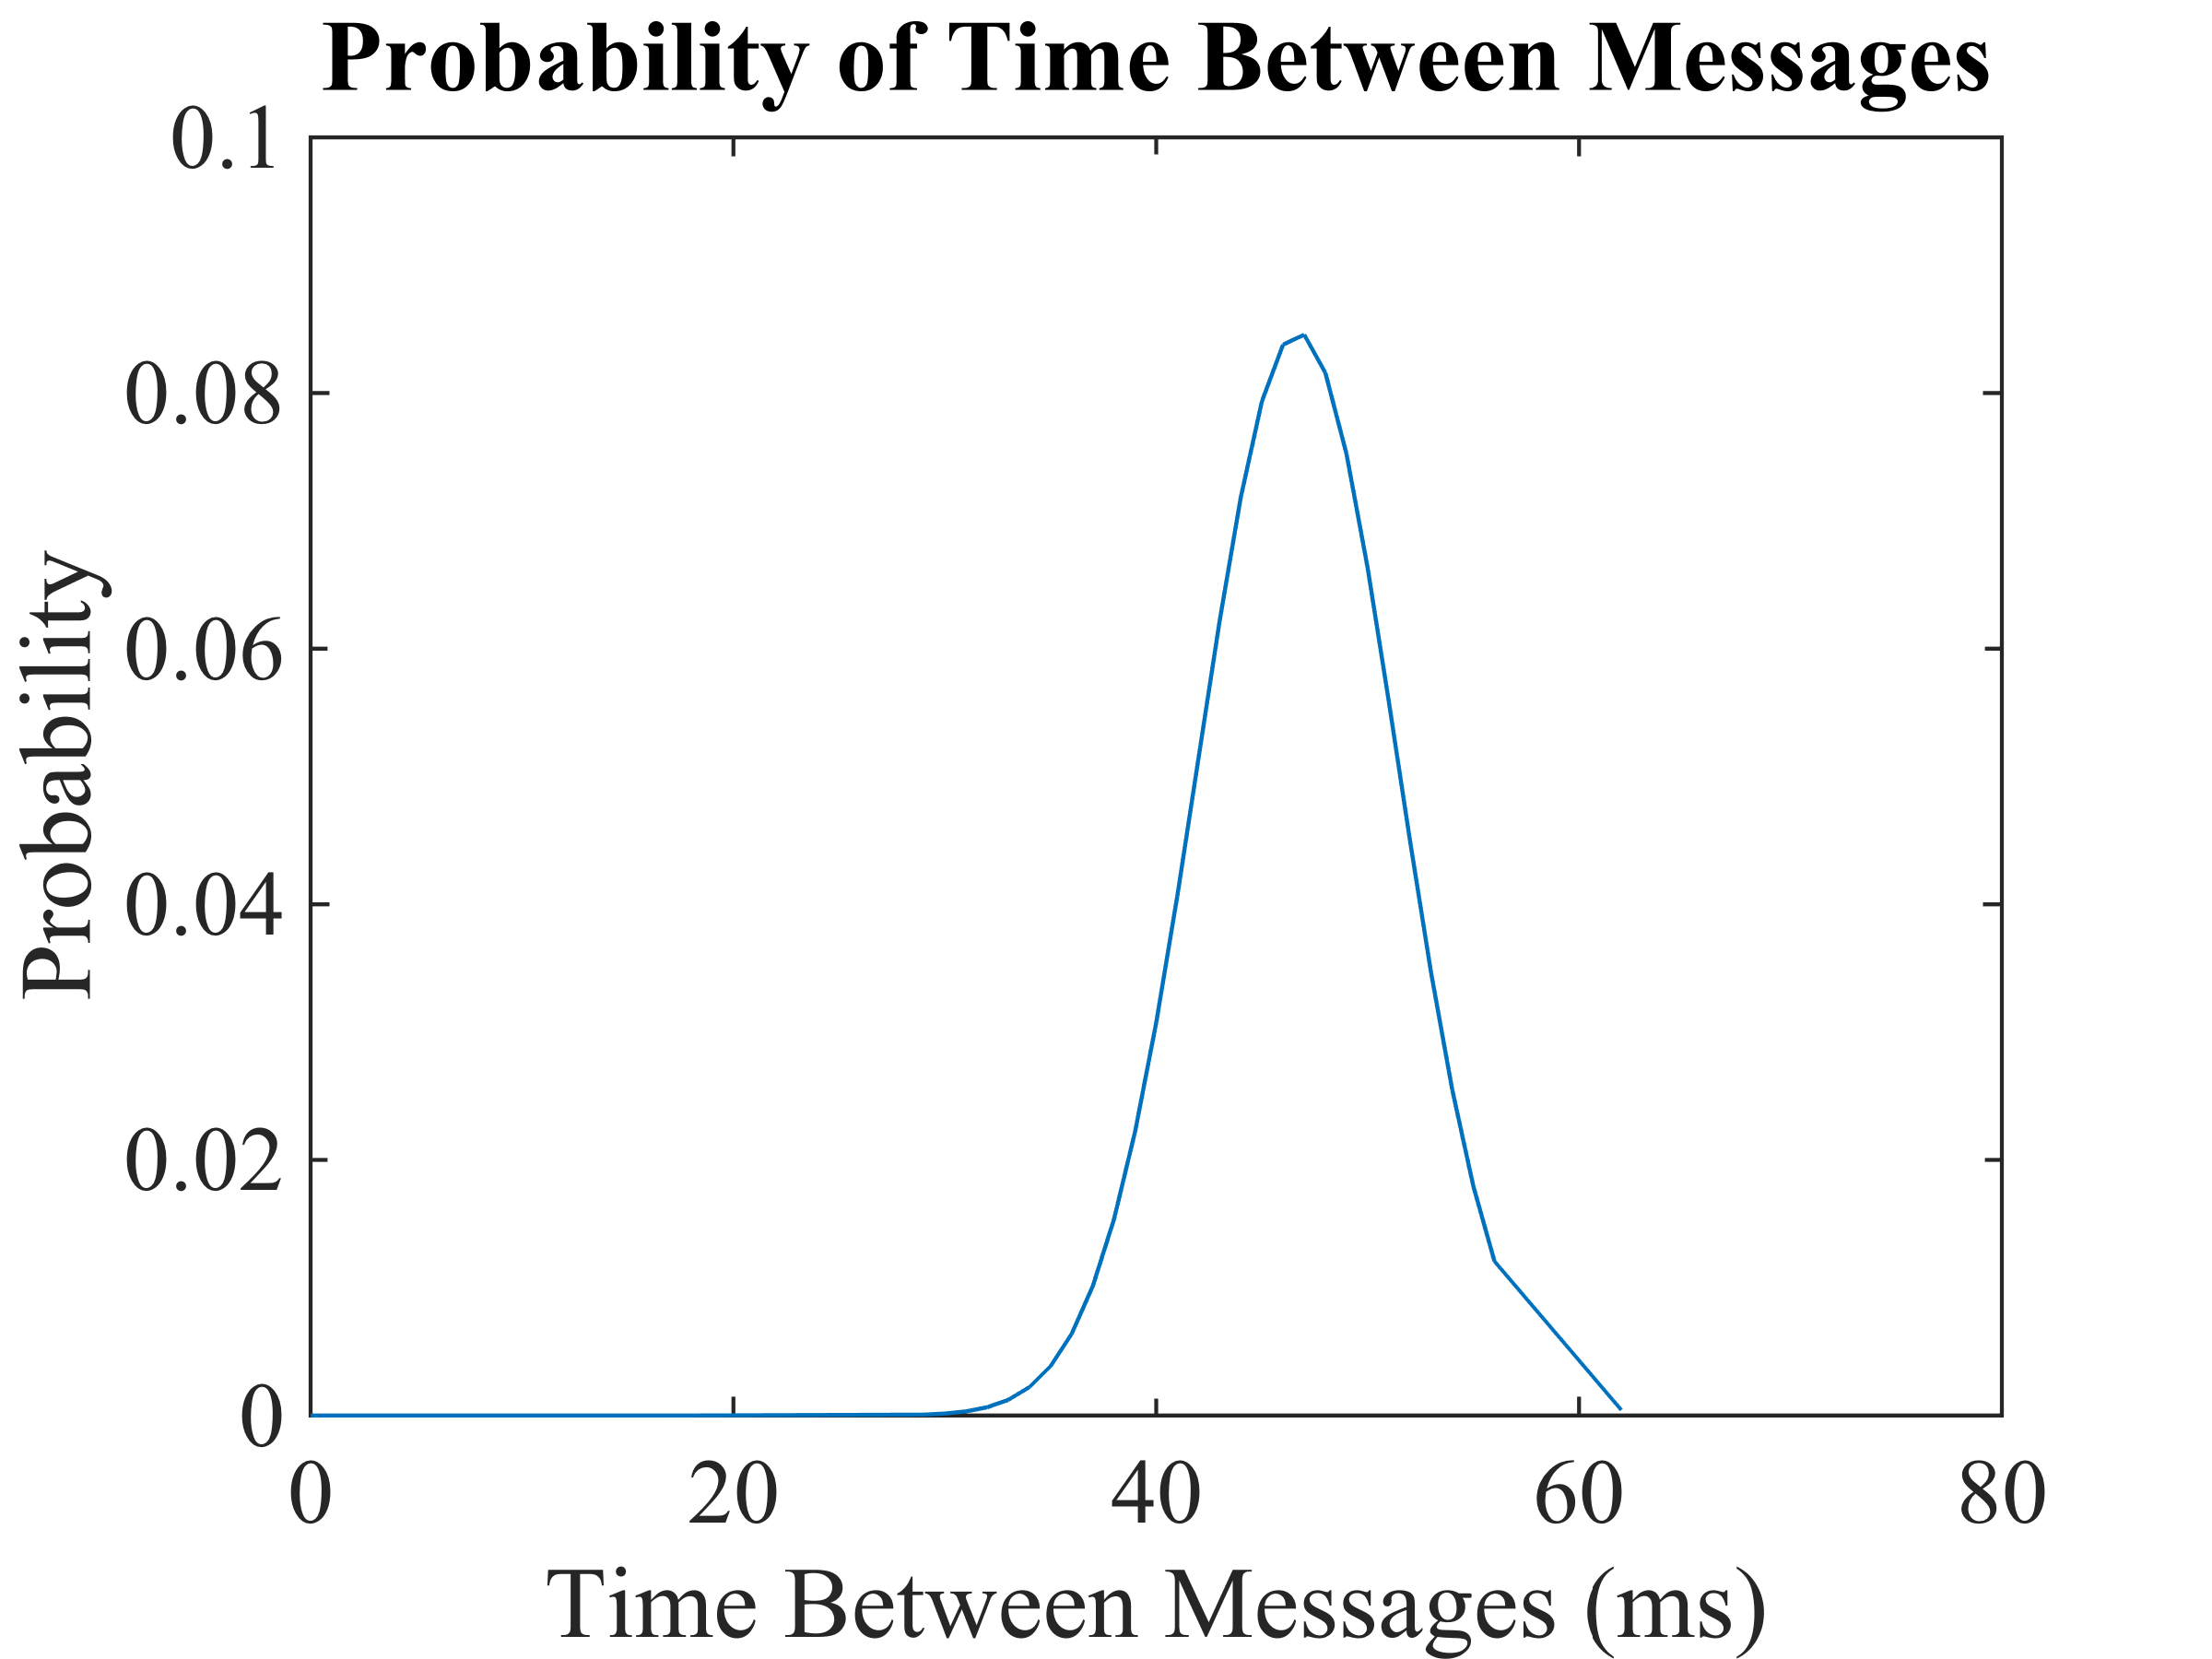
\includegraphics[width=\columnwidth]{figures/pdf.png}
		\caption{{\fontfamily{ptm}\selectfont Probability Density Function of Message Delay -- ECUs can easily be able to identify nodes spamming messages}}
	\end{figure}
	

There are some attacks that will defeat Mini-MAC. Perhaps the easiest way to defeat any CAN security mechanism is by flooding the bus. The attacker does not need to try and break any security, but by preventing ECUs from talking to each other, the attack succeeds as the car will not be able to function properly. Similarly, if an ECU is flashed with corrupted firmware, it does not need the correct group keys to launch an attack. It needs only to wait long enough to see the counters roll over. Most people keep the same automobile for many years, so even if this attack requires several years to gather enough information, it will still eventually succeed. Mini-MAC is useful against a resourceful attacker, but not a patient one.

\textcolor{red}{Note to ed: security analysis seems brief. still thinking on this.}